%% implemen.tex
%% $Id: implemen.tex 61 2012-05-03 13:58:03Z bless $
%%

\chapter{Implementierung}
\label{ch:Implementierung}
%% ==============================


Die Regeln wurden in der Programmiersprache \emph{C++} unter Verwendung der Bibliothek \emph{LEDA} \cite{manual} implementiert. Sie wurden bei der Anwendung jeweils solange wiederholt, bis sich am Graphen keine Änderung mehr ergab. 

%% ==============================
\section{Kronenregel}
%% ==============================
\label{ch:Implementierung:sec:Kronenregel}

Beim Austesten der Kronenregel hat sich gezeigt, dass die Auswahl des Matchings $M_{1}$ im in Kapitel \ref{ch:Grundlagen:sec:Kronenregel} dargestellten Algorithmus das Ergebnis der Reduktion in großem Maße beeinflusst, was bereits zuvor aufgefallen ist \cite{paper:7}. Dies ist bei der Implementierung für diese Arbeit dadurch aufgefallen, dass beim Anwenden an einem für die Kronenregel gut geeigneten Testgraphen zunächst keine Reduktion stattgefunden hat. Dieser ist in Abbildung \ref{fig:crown1} zu sehen. Um zu funktionieren, müssen die Kanten $(A,C), (D,E), (J,K), (L,B)$ für das Matching $M_{1}$ ausgewählt werden, da ansonsten zum Beispiel $K$ und $L$ nicht korrekt als Kopf der Krone, beziehungsweise nicht als der Menge $H$ zugehörig identifiziert werden.
\begin{figure}[htb]
\centering
  	{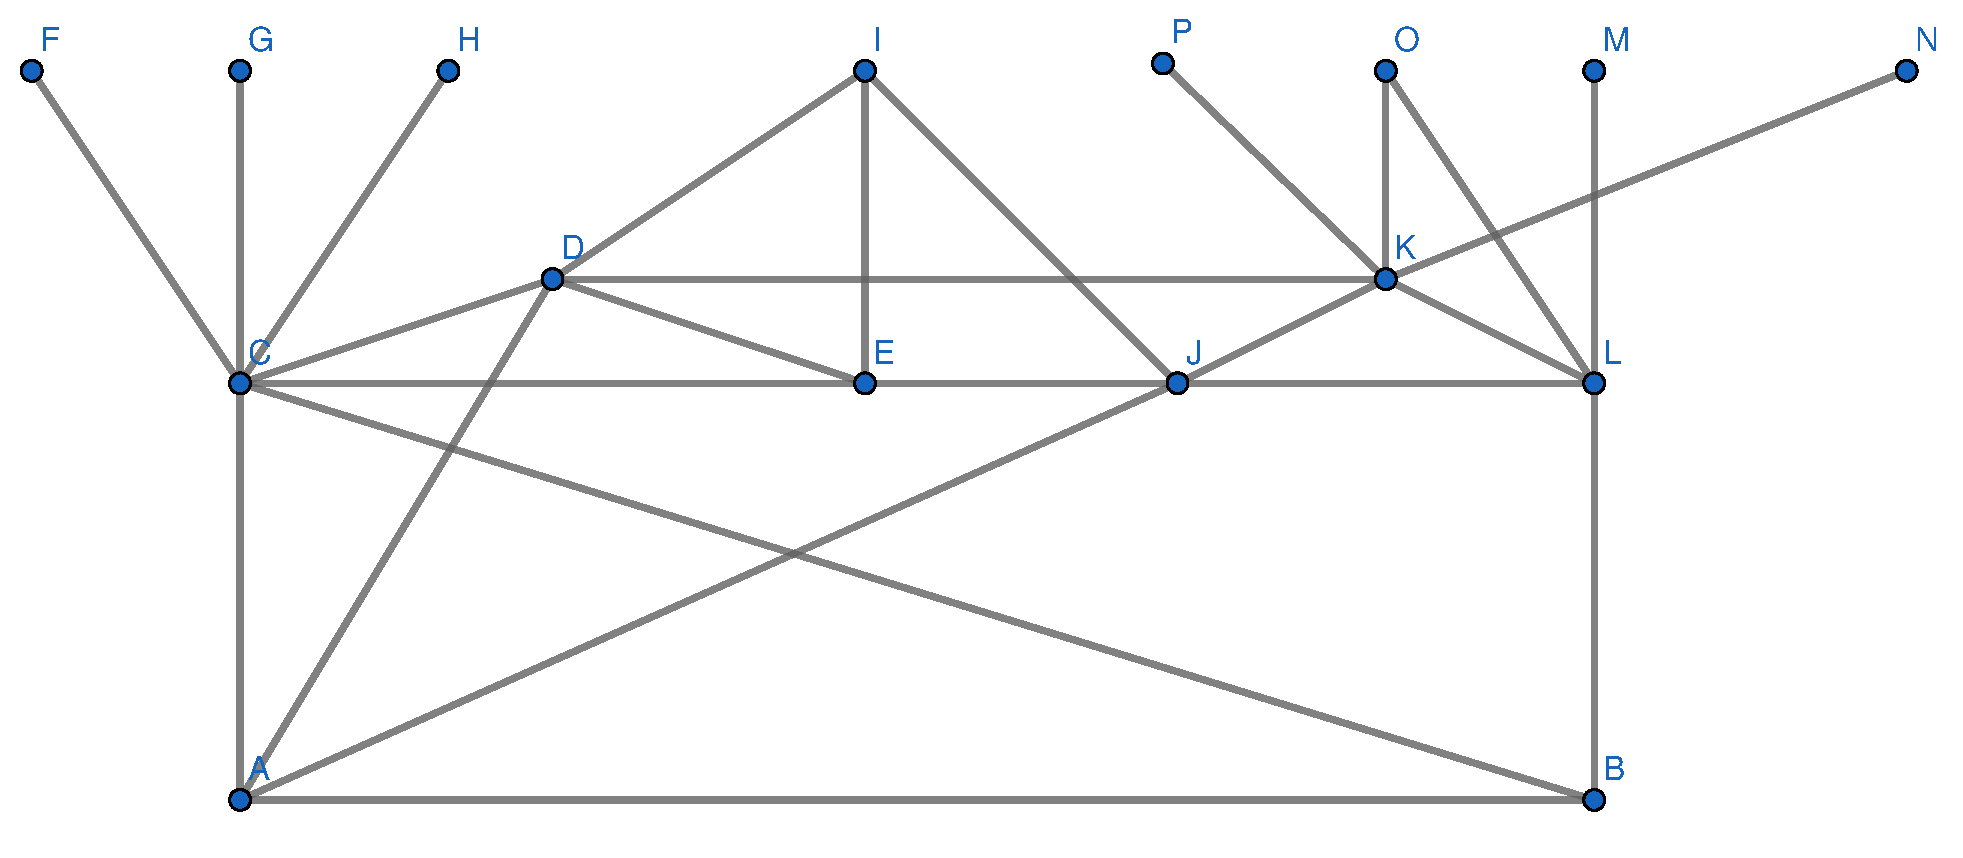
\includegraphics[width=.9\textwidth]{crown1Crop.pdf}}
	\caption{Beispielgraph für die Anwendung der Kronenregel\label{fig:crown1}}
\centering
\end{figure}
\begin{table}[htb]
\caption{Mindestens ein Knoten mit Einschränkung\label{tab:degreeOR}}
\vspace*{1em}
\centering

\bgroup
\def\arraystretch{1.3}%  1 is the default, change whatever you need

\begin{threeparttable}

\begin{tabular}[c]{lll}
	\hline
	\multicolumn{1}{c}{\textbf{Grad der Knoten}} & 
	\multicolumn{1}{c}{\textbf{Anwendungen}} & 
	\multicolumn{1}{c}{\textbf{Reduktion}} \\ 
	
	\hline

	keine Einschränkung&0.29&13.04\\
	>1&0.29 &13.04 \\
	>2&0.29 &13.22 \\
	>3& 0.27& 12.92 \\
	>4& 0.3& 13.71 \\
	>5& 0.31&13.38 \\
	>Größte Anzahl& 0.32&13.44 \\
	>Durchschnittliche Anzahl& 0.29&12.98 \\
	\hline
\end{tabular}
\begin{tablenotes}\footnotesize
\item \emph{Grad der Knoten} bezieht sich auf die Bedingung für die bevorzugte Auswahl der Kanten für $M_{1}$, bzw. dessen Knoten. \emph{Anwendung} und \emph{Reduktion} stellen jeweils den Durchschnittswert beim gesamten Testset dar.
\end{tablenotes}

\end{threeparttable}

\egroup

\end{table}


\begin{table}[h]
\caption{Beide Knoten mit Einschränkung\label{tab:degreeAND}}
\vspace*{1em}
\centering

\bgroup
\def\arraystretch{1.3}%  1 is the default, change whatever you need

\begin{threeparttable}
\begin{tabular}[c]{lll}
	\hline
	\multicolumn{1}{c}{\textbf{Grad der Knoten}} & 
	\multicolumn{1}{c}{\textbf{Anwendungen}} & 
	\multicolumn{1}{c}{\textbf{Reduktion}} \\ 
	
	\hline

	keine Einschränkung&0.29&13.04\\
	>1&0.36 &15.34 \\
	>2&0.41 &16.96 \\
	>3& 0.39& 16.52 \\
	>4& 0.4 &15.78 \\
	>5& 0.4 & 15.72\\
	>Größte Anzahl& 0.29 &13.06 \\
	>Durchschnittliche Anzahl& 0.46&19.77 \\
	\hline
\end{tabular}
\begin{tablenotes}\footnotesize
\item \emph{Grad der Knoten} bezieht sich auf die Bedingung für die bevorzugte Auswahl der Kanten für $M_{1}$, bzw. dessen Knoten. \emph{Anwendung} und \emph{Reduktion} stellen jeweils den Durchschnittswert beim gesamten Testset dar.
\end{tablenotes}

\end{threeparttable}

\egroup

\end{table}

Wenn nun beim Finden von $M_{1}$ zunächst bevorzugt Kanten mit Knoten höheren Grades vor den anderen betrachtet werden, können bessere Ergebnisse in der darauf folgenden Reduktion erzielt werden und die richtigen Kanten werden getroffen. Daraufhin wurde untersucht, wie die höhergradigen Knoten, beziehungsweise die dazugehörigen Kanten ausgewählt werden müssen. Auf der einen Seite (Tabelle \ref{tab:degreeOR}) wurden Kanten betrachtet, bei denen das Auswahlkriterium auf mindestens einen der Knoten zutrifft, auf der anderen Seite Kanten, bei denen beide Knoten die Bedingung erfüllen (Tabelle \ref{tab:degreeAND}). Die Einschränkungen \emph{Größte Anzahl} und \emph{Durchschnittliche Anzahl} ergeben sich jeweils aus der Menge an Knoten eines bestimmtes Grades. Bei Ersterem werden Knoten, deren Grad größer ist, als der, der im aktuellen Graphen am häufigsten vorkommt, bevorzugt. Bei Letzterem dementsprechend Knoten mit einem Grad, der größer ist, als der Durchschnittgrad im aktuellen Graphen. Diese Werte werden bei jeder Iteration des Algorithmus neu berechnet und passen sich dadurch während der Laufzeit an den Graphen an.\\ 
Generell wird eine bessere (größere) Reduktion mit der Kronenregel erreicht, wenn beim Matching $M_{1}$ zunächst Kanten betrachtet werden, bei denen die Einschränkung auf beide Knoten zutrifft. Die Reduktionsmenge bei Knoten mit $Grad>2$ erzeugt im Vergleich mit anderen statischen Werten das beste Ergebnis. Dies könnte damit zusammenhängen, dass bei den Graphen, bei denen diese Regel sehr effektiv ist, der durchschnittliche Grad der Knoten zwei ist und es sich damit um einen eher dünnen Graphen handelt. Vermutlich erzielt die Bevorzugung des durchschnittlichen Grades das beste Ergebnis, da sich dieser Wert mit jedem Durchlauf verändert.
Das Problem bei diesem Vorgehen ist, dass einfache Kronen ignoriert werden können, weshalb die Kombination mit der Grad$_{1}$-Regel vermutlich so gute Ergebnisse erzielt, wie in Kapitel \ref{ch:Analyse:sec:Anwendung} zu sehen ist.
\newpage




%% ==============================
\section{Nemhauser-Trotter-Regel}
%% ==============================
\label{ch:Implementierung:sec:Trott}

Bei der Umsetzung des Algorithmus' der Nemhauser-Trotter-Regel sind keine Besonderheiten aufgefallen, wie es bei der Kronenregel der Fall war. Für das Erstellen des bipartiten Graphen $B$ wurden zwei Referenzarrays angelegt, sodass für jeden Knoten aus $G$ das entsprechende Paar in $B$ gefunden werden konnte und anders herum, also für jeden Knoten aus $B$ das entsprechende Urbild aufgerufen werden konnte. Die weiteren Berechnungen konnten dann mithilfe der LEDA-Funktion MAX\_CARD\_BIPARTITE\_MATCHING aus mcb\_matching.h und LEDA-Iteratoren angestellt werden. Um zu überprüfen, ob der erstelle Graph $B$ tatsächlich bipartit ist und bei der Erstellung kein Fehler unterlaufen ist, wurde eigens eine entsprechende Funktion geschrieben, da LEDA eine solche nicht bereitstellt. In dieser Funktion wird getestet ob es möglich ist, die Knoten des Graphen in zwei Farben einzufärben, sodass keine zwei benachbarten Knoten die gleiche Farbe haben. Der Algorithmus funktioniert, wie folgt:
\begin{singlespace}
\begin{algorithm}[caption={Bipartit-Check}, label={alg4}]
Eingabe: Graph $G=(V,E)$ 
foreach $ v \in V$ do
  if Farbe[$v$]=leer then do
    Farbe[$v$] $\leftarrow$ Farbe$_{1}$    
    Queue.push($v$)
    while Queue.isNotEmpty do
      $v$ $\leftarrow$ Queue.pop
      if Farbe[$N(v)$]=leer oder Farbe[$N(v)$]=$\neg$Farbe[$v$] then do
        Farbe[$N(v)$] $\leftarrow$ $\neg$Farbe[$v$]
        Queue.push($N(v)$)
      else do
        return $G$ is nicht bipartit
      od 
    od
  od  
od
return $G$ ist bipartit
\end{algorithm}
\end{singlespace}
Die alles umschließende Schleife (Zeile 1) sorgt dafür, dass auch nicht verbundene Teile auf Bipartition überprüft werden. Genau genommen, überprüft der Algorithmus, ob in jedem nicht miteinander verbundenen Teil des Eingabegraphen eine Bipartition herrscht.

%% ==============================
%\section{Sonstige Algorithmen}
%% ==============================
%\label{ch:Implementierung:sec:Algo}
%Des weiteren wurden einige Hilfsalgorithmen implementiert:


%Um Informationen über den aktuellen Graphen zu sammeln, wurde eine recht einfache Methode umgesetzt, um einen Graphen auf Regularität zu überprüfen:
%\begin{singlespace}
%\begin{algorithm}[caption={Regulär-Check}, label={alg5}]
%Eingabe: Graph $G=(V,E)$ 
%p $\leftarrow$ zufälliger $v \in V$
%foreach $v \in V$ do
%  if Grad($v$) $\neq$ p do 
%    return $G$ ist nicht regulär
%  od
%od
%return $G$ ist regulär
%\end{algorithm}
%\end{singlespace}

%\begin{singlespace}
%\begin{algorithm}[caption={Regulär-Check}, label={alg4}]
%\end{algorithm}
%\end{singlespace}

%%% Local Variables: 
%%% mode: latex
%%% TeX-master: "thesis"
%%% End: 
